% !TEX program = lualatex
\documentclass[10pt, leqno]{ltjsarticle}
% \documentclass[10pt]{ltjsarticle} % 日本語をそのまま扱えるクラス
% \usepackage[margin=28mm]{geometry}
\usepackage{amsmath,amssymb,mathtools}
\usepackage{amsthm}
\usepackage{tikz}
\usetikzlibrary{arrows.meta,positioning,calc}

\usepackage[
  top=15mm,     % 上余白
  bottom=15mm,  % 下余白
  left=10mm,    % 左余白
  right=10mm,    % 右余白
  landscape,
  margin=10mm
]{geometry}
% \usepackage[landscape,margin=20mm]{geometry} % 余白はお好みで
\usepackage{paracol}
\columnratio{0.5,0.5}             % 左右を 1:1 に
\setlength{\columnseprule}{0.4pt} % 真ん中の縦線

\usepackage{titlesec}
\titleformat{\paragraph}
  {\normalfont\bfseries}
  {}      % ← 番号を空に
  {0pt}
  {}

  % 左揃えディスプレイ用ブロック
\newcommand{\Tharray}[1]{%
  \[
  \begin{array}{@{}l@{}} % 余白なしで左端に揃える
    #1
  \end{array}
  \]
}
% 上線を楽に:\ov{X} = \overline{X}
\newcommand{\ov}[1]{\overline{#1}}
% --- 左揃えの Thボディ用ヘルパ (プリアンブル or 本文先頭に一度だけ )---
\newenvironment{Thleft}[1][]{%
  % \begin{theorem}[#1]\mbox{}\\[-1.25ex]\begingroup
  \begin{theorem}[#1]\mbox{}\\[0ex]\begingroup
  \setlength{\arraycolsep}{0pt}% 式中の余白をタイトに
  \renewcommand{\arraystretch}{1.0}% 行間
  \noindent$\begin{array}{@{}l@{}}%
}{%
  \end{array}$\par\endgroup\end{theorem}%
}


% ---- 記号・マクロ ----
\newcommand{\xto}{\mathrel{\xrightarrow{}}}
\newcommand{\into}{\hookrightarrow}
\newcommand{\epi}{\twoheadrightarrow}
\newcommand{\pto}{\rightrightarrows}
\newcommand{\cls}[1]{\bigl(#1\bigr)}
\newcommand{\redjoin}{\wedge}
\newcommand{\shrink}{\phi}
\newcommand{\Ex}{E}        % suspension functor E
\newcommand{\Ox}{\Omega}   % loop functor Omega
\newcommand{\id}{\mathrm{id}}
% --- Toda bracket helpers ---
\newcommand{\toda}[1]{\{\,#1\,\}}              % {a,b,c}
\newcommand{\todai}[2][]{\{\,#2\,\}_{#1}}      % {a,b,c}_i   (#1 は添字, 空なら無し) 
\newcommand{\todas}[1]{\langle\,#1\,\rangle}
\newcommand{\gen}[1]{\{#1\}}       % ⟨generator⟩ 表記を { } で統一
\newcommand{\Ker}{\operatorname{Ker}}
\newcommand{\im}{\operatorname{Im}}
\newcommand{\hs}[2]{\bigl[#1,#2\bigr]}   % 一般のホモトピー集合
\newcommand{\pis}[2]{\pi_{#1}(#2)}       % 左が球面のときのホモトピー群
\newcommand{\pit}[2]{\pi_{#1}^{#2}}
\newcommand{\ext}[1]{\overline{#1}}     % extension
\newcommand{\coext}[1]{\widetilde{#1}}  % coextension
\newcommand{\z}{\mathbb{Z}}
\newcommand{\sq}[1]{Sq^{#1}}

% ---- theorem-like environments ----
\numberwithin{equation}{section}
\theoremstyle{plain}
\newtheorem{theorem}{Theorem}[section]
\newtheorem{lemma}[theorem]{Lemma}
\newtheorem{proposition}[theorem]{Proposition}
\newtheorem{corollary}[theorem]{Corollary}
\theoremstyle{definition}
\newtheorem{definition}[theorem]{Definition}
\newtheorem{example}[]{Example}
\newtheorem{notation}[theorem]{Notation}
\newtheorem{assumption}[theorem]{Assumption}
\theoremstyle{remark}
\newtheorem{remark}[]{Remark}

% \title{PART 1 \quad CHAPTER I\\[2mm] General Composition and Secondary Composition}
\author{}
\date{}

\begin{document}

\setcounter{section}{9}

% ==== CHAPTER IX p.89 ====

\section*{CHAPTER IX\\
Lemmas for Generators of \(\pis{n+11}{S^n;2}\)}

\begin{paracol}{2}

Th 7.4より，安定群 \(G_{11}\) の 2–primary 成分 \((G_{11};2)\) は 
\(\mathbb Z_8\) と同型で，\\
その生成元は \(\zeta=E^\infty\zeta_5\) である.\\
Toda bracket 
\(\todas{\nu,16\iota,\sigma}\)
を考える. これは,
\[
\begin{align*}
\nu\circ G_8+\sigma\circ G_4
& = \nu\circ (G_8;2)+\sigma\circ (G_4;2) \\
& = \{\,\nu\circ\varepsilon\,\}+\{\,\nu\circ\overline{\nu}\,\}+0 
&& \text{by Th7.1, Prop5.8,}\\
& = 0
&& \text{by (7.17), (7.18)}.
\end{align*}
\]
の coset であり，
したがって,  \(\todas{\nu,16\iota,\sigma}\) は単一元からなる. \\
\(\zeta\) と \(\zeta_5\) の定義から, 
\[
\begin{align*}
\zeta
= E^\infty\zeta_5
& \in E^\infty\toda{\nu_5,8\iota_8,E\sigma'}\\
& \subset \todas{E^\infty\nu_5, E^\infty8\iota_8, E^\infty\sigma'}\\
& = \todas{\nu,8\iota,2\sigma}
&& \text{by Lem5.14,}\\
& \subset \todas{\nu,16\iota,\sigma}
&& \text{by (3.5)}.  
\end{align*}
\]
よって, 次を得る：
\begin{equation}
% \noindent
% \textbf{(9.1).}\
\todas{\nu,8\iota,2\sigma} = \todas{\nu,16\iota,\sigma} = \zeta.
\end{equation}
また，(3.9) i) より, 
\begin{equation}
% \noindent
% \textbf{(9.2).}\
\todas{2\sigma,8\iota,\nu} = \todas{\sigma,16\iota,\nu} =  \zeta. 
\end{equation}
さらに,  (3.9) ii) を用いると, \\
\(
-\todas{\nu,8\iota,2\sigma}
+\todas{8\iota,2\sigma,\nu}
+\todas{2\sigma,\nu,8\iota}
\equiv 0
\)
\(\mod{\ \nu\circ G_8\ +\ 2\sigma\circ G_4\ +\ 8\iota\circ G_{11}\ } = 8G_{11}.\)\\
\((G_{11};2)\cong\mathbb Z_8\) なので, 
\(8G_{11}\) は \(G_{11}\) の奇数成分に一致する. 
(3.5) により, \\
\(\todas{2\sigma,\nu,8\iota}\ \equiv\ 2\todas{\sigma,\nu,8\iota}\ \ 
\mod\ 8G_{11} = 16G_{11}.\)
% ==== CHAPTER IX p.90 ====
よって, 次が従う：
\[
\begin{align*}
\todas{\nu,8\iota,2\sigma}
& \subset \todas{8\iota,2\sigma,\nu}+\todas{2\sigma,\nu,8\iota}+8G_{11} \\
& \subset \todas{8\iota,2\sigma,\nu}+2G_{11}.
\end{align*}
\]
\(2G_{11}/8G_{11}\) は \(2\zeta\) で生成されるので，
\(x \zeta \in \todas{8\iota,2\sigma,\nu}, \ \ (x:\text{ odd}).\)\\
(3.9) i) より, 
\(\todas{\nu,2\sigma,8\iota}=\todas{8\iota,2\sigma,\nu}.\)\\ 
さらに,  (3.5) から, 
\(\todas{8\iota,2\sigma,\nu}\supset\todas{16\iota,\sigma,\nu}\) で,
これらは, \(8G_{11} = 16G_{11}\) の coset .\\
よって,
\(\todas{8\iota, 2\sigma, \nu} = \todas{16\iota,\sigma,\nu}\). \\
(3.9) の i) により, 
\(\todas{\nu, \sigma, 16\iota} = \todas{16\iota, \sigma, \nu} .\)
以上から, 次を得る.
\begin{equation}
% \noindent
% \textbf{(9.3).}\
\todas{8\iota,2\sigma,\nu}
=\todas{16\iota,\sigma,\nu}
=\todas{\nu,\sigma,16\iota}
=\todas{\nu,2\sigma,8\iota}
= x\zeta+8G_{11}, \quad (x:\text{ odd}). 
\end{equation}

\switchcolumn

\noindent
\textbf{Th7.4.}\
% \(\pit{13}{2} \;=\; \gen{\eta_{2}\circ \varepsilon'} \;\oplus\; \gen{\eta_{2}^{2}\circ \mu_{4}}
%   \;\cong\; \mathbb Z_{4}\oplus\mathbb Z_{2},\)\\
% \(\pit{14}{3} \;=\; \gen{\mu'} \oplus \gen{\varepsilon_3\circ\nu_{11}} \oplus \gen{\nu'\circ\varepsilon_6}
%   \cong \mathbb{Z}_4 \oplus \mathbb{Z}_2 \oplus \mathbb{Z}_2,\)\\
% \(\pit{15}{4} = \gen{\nu_{4}\circ \sigma'\circ\eta_{14}} \oplus \gen{\nu_{4}\circ \overline{\nu}_{7}}
%   \oplus \gen{\nu_{4}\circ \varepsilon_{7}} \oplus \gen{E \mu'}
%   \oplus \gen{\varepsilon_4\circ\nu_{12}} \oplus \gen{E\nu'\circ\varepsilon_7}\)\\
% \(\qquad \cong \mathbb Z_{2}\oplus\mathbb Z_{2}\oplus\mathbb Z_{2}\oplus\mathbb Z_{4}
%   \oplus\mathbb Z_{2}\oplus\mathbb Z_{2},\)\\
% \(\pit{16}{5} \;=\; \gen{\zeta_{5}} \;\oplus\; \gen{\nu_{5}\circ \overline{\nu}_{8}}
%   \;\oplus\; \gen{\nu_{5}\circ \varepsilon_{8}}
%   \;\cong\; \mathbb Z_{8}\oplus\mathbb Z_{2}\oplus\mathbb Z_{2},\)
% \(\pit{17}{6} \;=\; \gen{\zeta_{6}} \;\oplus\; \gen{\overline{\nu}_{6}\circ \nu_{14}}
%   \;\cong\; \mathbb Z_{8}\oplus\mathbb Z_{4},\)\\
% \(\pit{n+11}{n} \;=\; \gen{\zeta_{n}} \;\oplus\; \gen{\overline{\nu}_{n}\circ \eta_{n+8}}
%   \;\cong\; \mathbb Z_{8}\oplus\mathbb Z_{2}\quad (n=7,8,9),\)\\
% \(\pit{n+11}{n} \;=\; \gen{\zeta_{n}}\ \cong\ \mathbb Z_{8}\quad (n=10,11, \ n\ge13),\) \\
% \(\pit{23}{12} = \gen{\Delta(\iota_{25})}\oplus\gen{\zeta_{12}}\cong\mathbb Z\oplus\mathbb Z_{8},\)\\
\((G_{11};2)=\gen{\zeta}\ \cong\ \mathbb Z_{8}.\)

\noindent
\textbf{Th7.1.}\
% \(\pit{10}{2}=0,\)\\
% \(\pit{n+8}{n}=\gen{\varepsilon_{n}}\cong\mathbb Z_{2}\quad (n=3,4,5),\)
% \(\pit{14}{6}=\gen{\ov\nu_{6}}\oplus\gen{\varepsilon_{6}}\cong\mathbb Z_{8}\oplus\mathbb Z_{2},\)\\
% \(\pit{15}{7}=\gen{\sigma'\circ\eta_{14}}\oplus\gen{\ov{\nu}_{7}}\oplus\gen{\varepsilon_{7}}\cong \mathbb Z_{2}\oplus\mathbb Z_{2}\oplus\mathbb Z_{2},\)\\
% \(\pit{16}{8}=\gen{\sigma_{8}\circ\eta_{15}}\oplus\gen{E\sigma'\circ\eta_{15}}\oplus\gen{\ov{\nu}_{8}}\oplus\gen{\varepsilon_{8}}\cong \mathbb Z_{2}\oplus\mathbb Z_{2}\oplus\mathbb Z_{2}\oplus\mathbb Z_{2},\)\\
% \(\pit{17}{9}=\gen{\sigma_{9}\circ\eta_{16}}\oplus\gen{\ov{\nu}_{9}}\oplus\gen{\varepsilon_{9}}\cong \mathbb Z_{2}\oplus\mathbb Z_{2}\oplus\mathbb Z_{2},\)\\
% \(\pit{n+8}{n}=\gen{\ov{\nu}_{n}}\oplus\gen{\varepsilon_{n}}\cong \mathbb Z_{2}\oplus\mathbb Z_{2}\quad (n\ge10),\)\\
\((G_{8};2)=\gen{\ov{\nu}}\oplus\gen{\varepsilon}\cong\mathbb Z_{2}\oplus\mathbb Z_{2}.\)

\noindent
\textbf{Prop5.8.}\
% \(\pi^{2}_{6}=\mathbb Z_4\gen{\eta_{2}\circ\nu'},\) \quad
% \(\pi^{3}_{7}=\mathbb Z_2\gen{\nu'\circ\eta_6},\) \quad
% \(\pi^{4}_{8}=\mathbb Z_2\gen{\nu_{4}\circ\eta_7}\oplus \mathbb Z_2\gen{E\nu'\circ\eta_7},\) \\
% \(\pi^{5}_{9}=\mathbb Z_2\gen{\nu_{5}\circ\eta_8},\) \quad
% \(\pi^{n}_{n+4}=0\ (n\ge6),\) \
\((G_{4};2)=0.\)

\noindent
\textbf{(7.17).}\
\(\Delta(\sigma_{11}) = \nu_5\circ\ov{\nu}_8 + \nu_5\circ\varepsilon_8,\
\nu_6\ov{\nu}_9 = \nu_6\circ\varepsilon_9 .\)

\noindent
\textbf{(7.18).}\
\(2\,\overline{\nu}_{6}\circ \nu_{14}
\ =\ \nu_{6}\circ\varepsilon_{9}
\ =\ \Delta(\nu_{13}^{2}).\)

\noindent
\textbf{(Def).}\
\(\zeta_{5}\ \in\ \todai[1]{\nu_{5},\,8\iota_{8},\,E\sigma'}
\ \in\ \pi^{5}_{16}/\bigl(\nu_{5}\circ E\pi^{7}_{15}\bigr)\).

\noindent
\textbf{Lem5.14.}\
\(\sigma_{8}\in\pi^{8}_{15}\ , \ \sigma'\in\pi^{7}_{14}\ , \ \sigma''\in\pi^{6}_{13}\) 
が存在して, 次を満たす. \\
\(H(\sigma_{8})=\iota_{15} \ ,\quad 2E\sigma_{8}=E^{2}\sigma',\)\\
\(H(\sigma')=\eta_{13} \ ,\quad 2\sigma'=E\sigma'',\)\\
\(H(\sigma'')=\eta_{11}^2 \ ,\quad 2\sigma''=E\sigma''' .\)

\noindent
\textbf{(3.5).}\
\(\text{0).}\ \todas{\alpha, \beta, \gamma}\equiv 0,
\ \text{ ($\alpha,\beta,\gamma$ のいずれかが $0$ のとき) }\).\\
\(\text{i).}\ \todas{\alpha, \beta, \gamma}\circ\delta
\subset \todas{\alpha, \beta, \gamma\circ\delta}\)\\
\(\text{ii).}\ \todas{\alpha, \beta, \gamma\circ\delta}
\subset \todas{\alpha, \beta\circ\gamma, \delta}\)\\
\(\text{iii).}\ \todas{\alpha\circ\beta, \gamma, \delta}
\subset \todas{\alpha, \beta\circ\gamma, \delta}\)\\
\(\text{iv).}\ \alpha\circ\todas{\beta, \gamma, \delta}
\subset (-1)^k\todas{\alpha\circ\beta, \gamma, \delta},\ \alpha\in G_k .\)

\noindent
\textbf{(3.9).}\
\(\text{i).}\ \todas{\alpha,\beta,\gamma}\ \subset\
(-1)^{hk+k\ell+\ell h+1}\ \todas{\gamma,\beta,\alpha},\)\\
\(\text{ii).}\ (-1)^{k\ell}\ \todas{\alpha,\beta,\gamma}\ +\
(-1)^{hk}\ \todas{\beta,\gamma,\alpha}\ +\
(-1)^{\ell k}\ \todas{\gamma,\alpha,\beta}\ \ni\ 0 .\)




\end{paracol}

\begin{paracol}{2}

\begin{equation}
% \noindent
% \textbf{(9.4).}\
\text{次の stable Toda bracket は, } 2G_{11} \text{ の coset.}
\qquad\qquad\qquad\qquad\qquad\qquad\qquad
\end{equation}
\[
\begin{aligned}
& \todas{\sigma,\eta^3,2\iota},\ 
\todas{2\iota,\eta^3,\sigma},\
\todas{\eta\circ\varepsilon,\eta,2\iota},\
\todas{2\iota,\eta,\eta\circ\varepsilon},\\
& \todas{\varepsilon,\eta^2,2\iota},\
\todas{2\iota,\eta^2,\varepsilon},\
\todas{\eta,\eta\circ\varepsilon,2\iota},\
\todas{2\iota,\eta\circ\varepsilon,\eta},\\
& \todas{\eta^2,\varepsilon,2\iota},\
\todas{2\iota,\varepsilon,\eta^2},\\
& \text{特に, } \todas{\nu^3,\eta,2\iota}=\todas{2\iota,\eta,\nu^3}=2G_{11}.
\end{aligned}
\]

\medskip
\noindent まず, 次に注意する：
\[
\begin{aligned}
&\sigma\circ G_4=\sigma\circ(G_4;2)=0,\\
&\varepsilon\circ G_2=\{\varepsilon\circ\eta^2\}=0,
\quad\text{by (7.10), (7.20)},\\
&\varepsilon\circ G_3=\{\varepsilon\circ\nu\}=0,
\quad\text{by (7.18)},\\
&\eta\circ G_{10}=\{\eta^2\circ\mu\}=\{4\zeta\}\subset 2G_{11},\\
&\eta^2\circ G_{9}
=\{\eta^3\circ\varepsilon\}+\{\eta^2\circ\nu^3\}+\{\eta^2\circ\mu\}
=0+0+\{4\zeta\}\subset 2G_{11},\\
&\nu^3\circ G_{2} = \{\nu^3\circ\eta^2\}=0.
\end{aligned}
\]
したがって, 上の Toda bracket は \(2G_{11}\) の coset である. 
(3.5) を用いると, 
\[
\todas{\eta\circ\varepsilon,\eta,2\iota}
=\todas{\varepsilon,\eta^2,2\iota},\qquad
\todas{\eta\circ\varepsilon,\eta,2\iota}
=\todas{\eta,\eta\circ\varepsilon,2\iota}
=\todas{\eta^2,\varepsilon,2\iota},
\]
などが従い，さらに,  (3.9) i) により, 
\[
\todas{\sigma,\eta^3,2\iota}
=\todas{2\iota,\eta^3,\sigma},\qquad
\todas{\eta\circ\varepsilon, \eta, 2\iota}
= \todas{2\iota, \eta, \eta\circ\varepsilon},
\]
\[
\todas{\varepsilon, \eta^2, 2\iota},
= \todas{2\iota, \eta^2, \varepsilon},\qquad
\todas{\eta, \eta\circ\varepsilon, 2\iota}
= \todas{2\iota, \eta\circ\varepsilon, \eta},
\]
\[
\todas{\eta^2, \varepsilon, 2\iota}
= \todas{2\iota, \varepsilon, \eta^2},\qquad
\todas{\nu^3,\eta,2\iota}
=\todas{2\iota,\eta,\nu^3}.
\]

% ==== CHAPTER IX p.91 ====

\noindent
\((G_{5};2)=0\) なので, 
\[
\nu^{2}\circ\todas{\nu,\eta,2\iota}\ \subset\ \nu^{2}\circ G_{5}=(G_{5};2)=0.
\]
(3.5) より, 
\[
\todas{\nu^{3},\eta,2\iota}\ \supset\ \nu^{2}\circ\todas{\nu,\eta,2\iota}=0.
\]
したがって,  \(\todas{\nu^{3},\eta,2\iota}=2G_{11}\) である. 最後に,
\[
\begin{align}
\todas{\eta\circ\varepsilon,\eta,2\iota}
&=\todas{\eta\circ\varepsilon,\eta,2\iota}+2G_{11}\\
&=\todas{\eta\circ\varepsilon,\eta,2\iota}+\todas{\nu^{3},\eta,2\iota}\\
&=\todas{\eta\circ\varepsilon + \nu^3, \eta, 2\iota}
&& \text{by (3.8),}\\
& =\todas{\sigma\circ\eta^{2},\eta,2\iota}
&& \text{by Lem6.4, 6.3,}\\
&=\todas{\sigma,\eta^{3},2\iota}.
\end{align}
\]
以上で (9.4) が示された. 

\switchcolumn

\noindent
\textbf{(7.10).}\
\(2(\nu_{5}\circ\sigma_{8})=\pm E^{2}\varepsilon',\
4(\nu_{n}\circ\sigma_{n+3})=\eta_{n}^{2}\circ\varepsilon_{n+2}\quad(n\ge5).\)

\noindent
\textbf{(7.20).}\
\(4\sigma_{10}\circ\nu_{17}
=2\sigma_{11}\circ\nu_{18}
=\sigma_{12}\circ\nu_{19}=0,\)\\
\(4\nu_{9}\circ\sigma_{12}
=2\nu_{10}\circ\sigma_{13}
=\nu_{11}\circ\sigma_{14}=0.\)

\noindent
\textbf{(7.18).}\
\(2\,\overline{\nu}_{6}\circ \nu_{14}
\ =\ \nu_{6}\circ\varepsilon_{9}
\ =\ \Delta(\nu_{13}^{2}).\)

\noindent
\textbf{(3.5).}\
\(\text{0).}\ \todas{\alpha, \beta, \gamma}\equiv 0,
\ \text{ ($\alpha,\beta,\gamma$ のいずれかが $0$ のとき) }\).\\
\(\text{i).}\ \todas{\alpha, \beta, \gamma}\circ\delta
\subset \todas{\alpha, \beta, \gamma\circ\delta}\)\\
\(\text{ii).}\ \todas{\alpha, \beta, \gamma\circ\delta}
\subset \todas{\alpha, \beta\circ\gamma, \delta}\)\\
\(\text{iii).}\ \todas{\alpha\circ\beta, \gamma, \delta}
\subset \todas{\alpha, \beta\circ\gamma, \delta}\)\\
\(\text{iv).}\ \alpha\circ\todas{\beta, \gamma, \delta}
\subset (-1)^k\todas{\alpha\circ\beta, \gamma, \delta},\ \alpha\in G_k .\)

\noindent
\textbf{(3.9).}\
\(\text{i).}\ \todas{\alpha,\beta,\gamma}\ \subset\
(-1)^{hk+k\ell+\ell h+1}\ \todas{\gamma,\beta,\alpha},\)\\
\(\text{ii).}\ (-1)^{k\ell}\ \todas{\alpha,\beta,\gamma}\ +\
(-1)^{hk}\ \todas{\beta,\gamma,\alpha}\ +\
(-1)^{\ell k}\ \todas{\gamma,\alpha,\beta}\ \ni\ 0 .\)

\noindent
\textbf{(3.8).}\
\(\todas{\alpha,\beta,\gamma}\ +\ \todas{\alpha,\beta,\gamma'}\ \supset\
\todas{\alpha,\beta,\,\gamma+\gamma'},\)\\
\(\todas{\alpha,\beta,\gamma}\ +\ \todas{\alpha,\beta',\gamma}\ =\
\todas{\alpha,\,\beta+\beta',\,\gamma},\)\\
\(\todas{\alpha,\beta,\gamma}\ +\ \todas{\alpha',\beta,\gamma}\ \supset\
\todas{\,\alpha+\alpha',\,\beta,\,\gamma}.\)

\noindent
\textbf{Lem6.4.}\
\(\eta_9\circ \sigma_{10}\ =\ \overline\nu_9+\varepsilon_9,
\quad \eta_n\circ \sigma_{n+1}\ =\ 
\sigma_n \circ\eta_{n+7}\ =\
\overline\nu_n+\varepsilon_n,\ \text{ for } n\ge10.\)

\noindent
\textbf{Lem6.3.}\
\(n\ge6\) に対し,
\(\overline\nu_n\circ \eta_{n+8}\ 
=\ \eta_n\circ \overline\nu_{n+1}\ =\ \nu_n^{3},
\ (\nu_n^{3}:=\nu_n\circ \nu_{n+3}\circ \nu_{n+6}).\)



\end{paracol}

\begin{paracol}{2}

\begin{lemma}
% \noindent
% \textbf{(Lem9.1.)}\
\[
\begin{aligned}
&\todas{\sigma,\eta^{3},2\iota}=\todas{2\iota,\eta^{3},\sigma}=\zeta+2G_{11},\\
&\todas{\eta\circ\varepsilon,\eta,2\iota}=\todas{2\iota,\eta,\eta\circ\varepsilon}=\zeta+2G_{11},\\
&\todas{\varepsilon,\eta^{2},2\iota}=\todas{2\iota,\eta^{2},\varepsilon}=\zeta+2G_{11},\\
&\todas{\eta,\eta\circ\varepsilon,2\iota}=\todas{2\iota,\eta\circ\varepsilon,\eta}=\zeta+2G_{11},\\
&\todas{\eta^{2},\varepsilon,2\iota}=\todas{2\iota,\varepsilon,\eta^{2}}=\zeta+2G_{11}.
\end{aligned}
\]
\end{lemma}

\noindent
\textbf{Proof.}\
(9.4) より，
\(\todas{\eta\circ\varepsilon,\eta,2\iota}\not\equiv0\pmod{2G_{11}}\) 
を示せば十分である. \\
\(\todas{\eta\circ\varepsilon,\eta,2\iota}\equiv0\pmod{2G_{11}}\) 
と仮定して矛盾を導く. 

\(n\) を十分大きく (例えば \(n>13\)) とる. 
\(\todas{\eta\circ\varepsilon,\eta,2\iota}\equiv0\pmod{2G_{11}}\) 
と仮定すると，
\[
0 \in \toda{\eta_{n}\circ\varepsilon_{n+1},\,\eta_{n+9},\,2\iota_{n+10}}.
\] 
\(K_{1}:=S^{n+9}\cup_{\eta_{n+9}} e^{n+11}\) 
とすると, Prop 1.7により,\\
\(
\alpha_{1}\in[K_{1}, S^{n}]:\eta_{n}\circ\varepsilon_{n+1} \text{ の extension},\
\beta_{1}\in\pi_{n+11}(K_{1}):2\iota_{n+10} \text{ の coextension},
\)\\
が存在し, 
\(\alpha_1\circ\beta_1 = 0\)
を満たす.\\
\(H_{2}(\eta_{n+9})\neq0\) なので，
\(K_{1}\) では \(Sq^{2}\neq0\). \\
\(L_{1} := K_{1}\cup_{\beta_1} e^{n+12} 
= S^{n+9} \cup_{\eta_{n+9}} e^{n+11} \cup_{\beta_1} e^{n+12}\)
とする.\\
\(\alpha_{1}\circ\beta_{1}=0\) なので,  \(\alpha_{1}\) の extension 
\(\widetilde{\alpha}\in[L_{1}, S^{n}]\) が存在し，\\
その代表を 
\(f_{1}:L_{1}\to S^{n}\) 
とする. \\
Lem 8.2から, 
\(Sq^{3}=Sq^{1}Sq^{2}\neq0 \ \text{ in }\ L_1.\)\\
同様に，(9.4) の \(\todas{\nu^{3},\eta,2\iota}\equiv 0\) から, 
\[
L_{2}=S^{n+9}\cup_{\eta_{n+9}} e^{n+11}\cup e^{n+12}
\]
を構成でき，
% ==== CHAPTER IX p.92 ====
\[
Sq^3=Sq^1Sq^2\ne0 \ \text{ in } \ L_2.
\]
ここで, 写像
\[
f_2:L_2\to S^n
\]
で，その $S^{n+9}$ 上の制限 \(f_2|{S^{n+9}}\) が,
$\nu_n^3$ を表すようなものが存在する. さらに, 
\[
f_3:S^{n+9}\to S^n
\]
を, $\mu_n$ を表す写像とする. このとき, $f_1,f_2,f_3$ から, 
次の写像を定義する.
\[
f:= f_1\vee f_2\vee f_3 :L_1\vee L_2\vee S^{n+9}\longrightarrow S^n.
\]
Th 7.2より，
$\eta_n\circ\varepsilon_{n+1}$，$\nu_n^3$，$\mu_n$ が,
$\pi_{n+9}(S^n)$ の 2-成分を生成するので，
\[
f_*:\ \pi_{n+9}(L_1\vee L_2\vee S^{n+9})\ \longrightarrow\ \pi_{n+9}(S^n)
\]
は, その 2-成分 \(\pis{n+9}{S^n;2}\) の上に全射で写る. 

\switchcolumn

\noindent
\textbf{(9.4).}\
次の stable Toda bracket は, \(2G_{11}\) の coset.\\
\(\todas{\sigma,\eta^3,2\iota},\ 
\todas{2\iota,\eta^3,\sigma},\
\todas{\eta\circ\varepsilon,\eta,2\iota},\
\todas{2\iota,\eta,\eta\circ\varepsilon},\)\\
\(\todas{\varepsilon,\eta^2,2\iota},\
\todas{2\iota,\eta^2,\varepsilon},\
\todas{\eta,\eta\circ\varepsilon,2\iota},\
\todas{2\iota,\eta\circ\varepsilon,\eta},\)\\
\(\todas{\eta^2,\varepsilon,2\iota},\
\todas{2\iota,\varepsilon,\eta^2},\)\\
特に, \(\todas{\nu^3,\eta,2\iota}=\todas{2\iota,\eta,\nu^3}=2G_{11}.\)

\noindent
\textbf{Prop1.7.}\
\(\todai[n]{\alpha, E^n\beta, E^n\gamma}
= (-1)^n\gen{\overline{\alpha}\circ E^n\widetilde{\gamma}}\).

\noindent
\(S^n\xleftarrow{\alpha_1}
K_1 = S^{n+9}\cup_{\eta_{n+9}}e^{n+1} \xleftarrow{\beta_1}
S^{n+1}\).

\noindent
\textbf{Lem8.2.}\
$H_2(\beta)\ne0$ と仮定する. このとき,\\
\(\sq{i}(u_{n+1}) = u_{n+i+1}
\quad\text{in} \ \ H^\ast (X\cup e^{n+1}\cup_f CS^{n+i}; \z_2).\)\\
ここで, $u_{n+i+1}$ は $u_{n+1}$ と同様に, $CS^{n+i}$ により表される. 

\noindent
\textbf{Th7.2.}\
% \(\pit{11}{2}=\gen{\eta_{2}\circ\varepsilon_{3}}\cong\mathbb Z_{2},\)\\
% \(\pit{12}{3}=\gen{\mu_{3}}\oplus\gen{\eta_{3}\circ\varepsilon_{4}}\cong\mathbb Z_{2}\oplus\mathbb Z_{2},\)\\
% \(\pit{n+9}{n}=\gen{\nu_{n}^{3}}\oplus\gen{\mu_{n}}\oplus\gen{\eta_{n}\circ\varepsilon_{n+1}}
% \cong\mathbb Z_{2}\oplus\mathbb Z_{2}\oplus\mathbb Z_{2}\quad (n=4,5,6),\)
% \(\pit{16}{7}=\gen{\sigma'\circ\eta_{14}^{\,2}}\oplus\gen{\nu_{7}^{3}}\oplus\gen{\mu_{7}}\oplus\gen{\eta_{7}\circ\varepsilon_{8}}
% \cong\mathbb Z_{2}\oplus\mathbb Z_{2}\oplus\mathbb Z_{2}\oplus\mathbb Z_{2},\)\\
% \(\pit{17}{8}=\gen{\sigma_{8}\circ\eta_{15}^{\,2}}\oplus\gen{E\sigma'\circ\eta_{15}^{\,2}}\oplus\gen{\nu_{8}^{3}}\oplus\gen{\mu_{8}}\oplus\gen{\eta_{8}\circ\varepsilon_{9}}
% \cong\mathbb Z_{2}\oplus\mathbb Z_{2}\oplus\mathbb Z_{2}\oplus\mathbb Z_{2}\oplus\mathbb Z_{2},\)\\
% \(\pit{18}{9}=\gen{\sigma_{9}\circ\eta_{16}^{\,2}}\oplus\gen{\nu_{9}^{3}}\oplus\gen{\mu_{9}}\oplus\gen{\eta_{9}\circ\varepsilon_{10}}
% \cong\mathbb Z_{2}\oplus\mathbb Z_{2}\oplus\mathbb Z_{2}\oplus\mathbb Z_{2},\)\\
% \(\pit{19}{10}=\gen{\Delta(\iota_{21})}\oplus\gen{\nu_{10}^{3}}\oplus\gen{\mu_{10}}\oplus\gen{\eta_{10}\circ\varepsilon_{11}}
% \cong\mathbb Z\oplus\mathbb Z_{2}\oplus\mathbb Z_{2}\oplus\mathbb Z_{2},\)\\
\(\pit{n+9}{n}=\gen{\nu_{n}^{3}}\oplus\gen{\mu_{n}}\oplus\gen{\eta_{n}\circ\varepsilon_{n+1}}
\cong\mathbb Z_{2}\oplus\mathbb Z_{2}\oplus\mathbb Z_{2}\quad (n\ge11),\)\\
\((G_{9};2)=\gen{\nu^{3}}\oplus\gen{\mu}\oplus\gen{\eta\circ\varepsilon}\cong\mathbb Z_{2}\oplus\mathbb Z_{2}\oplus\mathbb Z_{2}.\)




\end{paracol}

\begin{paracol}{2}

次に, [23] の結果を用いる. \\
$K_9$ を CW 複体で，その $(n+9)$–skeleton が $S^n$，\\
かつ $\pi_i(K_9)=0\ (i\ge n+9)$ をみたすものとする. \\
このとき, [23] の Prop 4.9より, 
\begin{equation}\label{eq:K9coh}
% \noindent
% \textbf{(9.5).}\
H^{n+10}(K_9;\mathbb Z_2)\ \cong\ 
\z_2\gen{h_9}\oplus\z_2\gen{i_9}\oplus\z_2\gen{j_9},
\end{equation}
\[
Sq^2 h_9 = Sq^3 i_9 = 0.
\]

\[
S := \Omega(K_9; K_9, S^n),
\]
とする.
各 path の始点を対応させることにより, 
次の Serre fibration を得る [13].
\[
p':S\longrightarrow K_9.
\]
$S^n$ を \(S\) の deformation retract と考えることができる.\\
また, この retraction によって, 
\(p'\) は  $S^n\hookrightarrow K_9$ に同値である. \\
この fibration の, 基点 $e_0$ 上の fiber $Y=p'^{-1}(e_0)$ は,
$e_0$ を始点にもつ path からなる.\\
fibration のホモトピー完全列から，
\[
i_*:\pi_i(Y)\to\pi_i(S)
\ \text{は,}\ i>n+8\ \text{で同型，}\qquad
\pi_i(Y)=0\ \text{for }\ i\le n+8,
\]
であることは容易に確かめられる. \\
したがって,  $Y$ は $S^n$ 上の $(n+8)$–連結 fiber 空間である. \\
各 path の終点を対応させることで, fibration
\[
p:Y\longrightarrow S^n
\]
を得る. これは, retraction により, 
$i:Y\hookrightarrow S$ に同値である. 
ゆえに,
\[
p_*:\pi_i(Y)\longrightarrow \pi_i(S^n)
\]
は, $i>n+8$ で同型 である. 

さらに, [13] Chapter III の Prop 5 より，\\
fibration $p':S\to K_9$ に付随する
コホモロジー群の次の完全列が得られる：
\[
\cdots\longrightarrow H^{i}(S; \z_2)
\xrightarrow{i^*}H^i(Y; \z_2)
\xrightarrow{\Sigma} H^{*}(K_9; \z_2)
\xrightarrow{p'^*}H^{*}(S; \z_2)
\xrightarrow{}\cdots,\ (i<2n+8),
\]
% ==== CHAPTER IX p.93 ====
% 直前からのコホモロジー完全列
ここで $\Sigma$ は懸垂準同型である. \\
$H^i(S;\mathbb Z_2)=0\ (i>n)$ なので，
$n<i<2n+8$ に対して, $\Sigma$ は同型となる. \\
$\Sigma$ は $Sq$ と可換なので，(9.5) から,
\begin{equation}\label{eq:Ycoh}
% \noindent
% \textbf{(9.6).}\
H^{n+9}(Y;\mathbb Z_2)\ \cong\ \mathbb Z_2\oplus\mathbb Z_2\oplus\mathbb Z_2.
\end{equation}

\switchcolumn

\noindent
\textbf{Lem9.1.}\
\(\todas{\sigma,\eta^{3},2\iota}=\todas{2\iota,\eta^{3},\sigma}=\zeta+2G_{11},\)\\
\(\todas{\eta\circ\varepsilon,\eta,2\iota}=\todas{2\iota,\eta,\eta\circ\varepsilon}=\zeta+2G_{11},\)\\
\(\todas{\varepsilon,\eta^{2},2\iota}=\todas{2\iota,\eta^{2},\varepsilon}=\zeta+2G_{11},\)\\
\(\todas{\eta,\eta\circ\varepsilon,2\iota}=\todas{2\iota,\eta\circ\varepsilon,\eta}=\zeta+2G_{11},\)\\
\(\todas{\eta^{2},\varepsilon,2\iota}=\todas{2\iota,\varepsilon,\eta^{2}}=\zeta+2G_{11}.\)

\noindent
\cite{Toda1958a}
H.~Toda,
\newblock On exact sequences in Steenrod algebra mod 2,
\newblock Memoirs Univ. of Kyoto, {\bf 31} (1958), 33--64.

\noindent
\cite{Serre1951}
J.-P.~Serre,
\newblock Homologie singulière des espaces fibrés,
\newblock Ann. of Math., {\bf 54} (1951), 425--505.



\end{paracol}

\begin{paracol}{2}

\noindent
\(H^{n+9}(Y;\z_2)\) は, $Sq^3=Sq^1Sq^2$ で消える
$\z_2\oplus\z_2$ に同型な部分群を含む. 
\[
f=f_1\vee f_2\vee f_3 :L_1\vee L_2\vee S^{n+9}\to S^n
\]
を考える.\\
cell 複体 $L_1\vee L_2\vee S^{n+9}$ の $(n+8)$–skeleton は自明なので，
次の写像が存在する.
\[
F:L_1\vee L_2\vee S^{n+9}\to Y,\quad p\circ F = f.
\]
次の可換図式を考える：
\[
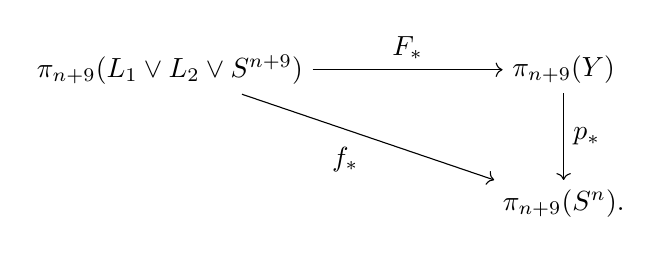
\begin{tikzpicture}[baseline=(current bounding box.center)]
\node (A) at (0,1.7) {$\pis{n+9}{L_1\vee L_2\vee S^{n+9}}$};
\node (B) at (5,1.7) {$\pis{n+9}{Y}$};
\node (C) at (5,0) {$\pis{n+9}{S^n}.$};
\draw[->] (A) -- node[above] {$F_*$} (B);
\draw[->] (A) -- node[below left] {$f_*$} (C);
\draw[->] (B) -- node[right] {$p_*$} (C);
\end{tikzpicture}
\]
$p_*$ は同型で，$f_*$ は 2-成分の全射なので，$F_*$ も 2-成分で全射である. \\
$Y$ と $L_1\vee L_2\vee S^{n+9}$ は $(n+8)$–連結なので，
\[
F_* : H_{n+9}(L_1\vee L_2\vee S^{n+9}; \z_2)
\longrightarrow H_{n+9}(Y; \z_2)
\]
は全射.
双対性により, 
\[
F^*:H^{n+9}(Y;\mathbb Z_2)\longrightarrow
H^{n+9}(L_1\vee L_2\vee S^{n+9};\mathbb Z_2)
\]
は単射である. 明らかに,
\[
H^{n+9}(L_1\vee L_2\vee S^{n+9};\mathbb Z_2)\cong\mathbb Z_2\oplus\mathbb Z_2\oplus\mathbb Z_2 .
\]
よって, \(F^*\) は同型.
さらに,  $L_1,L_2$ 上で, \(Sq^{3}\ne0\),
\(S^{n+9}\) 上で, $Sq^3=0$ なので, 
\[
Sq^3 H^{n+9}(L_1\vee L_2\vee S^{n+9};\mathbb Z_2)\cong\mathbb Z_2\oplus\mathbb Z_2 .
\]
よって, (9.6) から, 
\[
Sq^3 H^{n+9}(Y;\mathbb Z_2)\ \cong\ \z_2\ \text{or}\ 0.
\]
しかし, これらの結果は，次の図式の可換性と矛盾する：
\[
\begin{array}{ccc}
H^{n+9}(Y;\mathbb Z_2) & \xrightarrow{\ F^*\ } & H^{n+9}(L_1\vee L_2\vee S^{n+9};\mathbb Z_2)\\[2pt]
\bigg\downarrow Sq^3 & & \bigg\downarrow Sq^3\\[-2pt]
H^{n+12}(Y;\mathbb Z_2) & \xrightarrow{\ F^*\ } & H^{n+12}(L_1\vee L_2\vee S^{n+9};\mathbb Z_2).
\end{array}
\]
したがって, 仮定 $\langle\eta\circ\varepsilon,\eta,2\iota\rangle=0$ は矛盾を生み，
 Lem は証明された. 
\qed

\switchcolumn

\noindent
\textbf{Lem9.1.}\
\(\todas{\sigma,\eta^{3},2\iota}=\todas{2\iota,\eta^{3},\sigma}=\zeta+2G_{11},\)\\
\(\todas{\eta\circ\varepsilon,\eta,2\iota}=\todas{2\iota,\eta,\eta\circ\varepsilon}=\zeta+2G_{11},\)\\
\(\todas{\varepsilon,\eta^{2},2\iota}=\todas{2\iota,\eta^{2},\varepsilon}=\zeta+2G_{11},\)\\
\(\todas{\eta,\eta\circ\varepsilon,2\iota}=\todas{2\iota,\eta\circ\varepsilon,\eta}=\zeta+2G_{11},\)\\
\(\todas{\eta^{2},\varepsilon,2\iota}=\todas{2\iota,\varepsilon,\eta^{2}}=\zeta+2G_{11}.\)

\noindent
\(L_1 = L_2 = S^{n+9}\cup_{\eta_{n+9}}e^{n+1}\cup_{\beta_i}e^{n+12}\).

\noindent
\textbf{(9.6).}\
\(H^{n+9}(Y;\mathbb Z_2)\ \cong\ \mathbb Z_2\oplus\mathbb Z_2\oplus\mathbb Z_2.\)





\end{paracol}

\begin{paracol}{2}

\begin{lemma}[]\label{lem:9.2}
% \noindent
% \textbf{Lem9.2.}\
\qquad\qquad\qquad\qquad\qquad
\(\nu_7\circ \zeta_{10}\;=\;\Ex^{2}\sigma'''\circ \sigma_{14}\, .\)
\end{lemma}

\noindent
\textbf{Proof.}\
$\Ex^\infty:\pi_{22}(S^{11})\to G_{11}$ を考える. \\
Th 7.4より, これは 2-成分に関して同型である.\\
奇数成分で, $\pi_{22}(S^{11})$ は安定群と一致する (cf.\ (13.5)) ので,
\(E^\infty\) は同型である. \\
(7.20) より,  $\nu_{11}\circ \sigma_{14}=0$．したがって,  Toda bracket 
\[
  \toda{\,8\iota_{11},\,\nu_{11},\,\sigma_{14}\,}
\]
が定義でき，$\Ex^\infty$ により, 
$\todas{8\iota,\nu,\sigma}$ の上に写る. \\
\(\todas{8\iota, \nu, \sigma}\)
は, \(8G_{11} + \sigma\circ G_4 = 8G_{11}\) の coset である.\\
(3.5) により, 
\[
\todas{8\iota, \nu, \sigma} 
\subset\todas{2\iota, 4\nu, \sigma}
= \todas{2\iota, \eta^3, \sigma}.
\]
Lem 9.1より, 奇数 $x$ が存在して,
\[
x\,\zeta\in \todas{8\iota,\nu,\sigma}.
\]
よって, 
\[
x\,\zeta_{11}\in \toda{8\iota_{11},\nu_{11},\sigma_{14}}.
\]
\[
\begin{aligned}
  \Ex(x\,\nu_7\circ \zeta_{10})
  & = \nu_8\circ x\,\zeta_{11}
  \in \nu_8\circ \toda{8\iota_{11},\nu_{11},\sigma_{14}}\\
  & = - \toda{\nu_8,8\iota_{11},\nu_{11}} \circ \sigma_{15}
  && \text{by Prop1.4.}\\
  \Ex(\Ex^{2}\sigma'''\circ \sigma_{14})
  & \in \Ex^{3}\toda{\nu_{5},\,8\iota_{8},\,\nu_{8}}\circ \sigma_{15}
  && \text{by Lem5.13,}\\
  & \subset \toda{\nu_8,8\iota_{11},\nu_{11}}\circ \sigma_{15}
  && \text{by Prop1.3.}
\end{aligned}
\]
\(-\toda{\nu_8,8\iota_{11},\nu_{11}}\circ \sigma_{15}\)
は, 次の群の coset である.
\[
\begin{aligned}
  \nu_8\circ \pi_{15}(S^{11})\circ \sigma_{15}
  & = \nu_8\circ \pit{15}{11}\circ\sigma_{15}
  && \text{by (4.7)}\\
  & = 0
  && \text{by Prop5.8.}
\end{aligned}
\]
したがって, 
\[
  \Ex(x\,\nu_7\circ \zeta_{10})
  \;=\; \Ex(\Ex^{2}\sigma'''\circ \sigma_{14}).
\]
Lem 4.5 により, 
$\Ex:\pi_{21}(S^{7})\to \pi_{22}(S^{8})$ は単射なので，
\[
  x\,\nu_7\circ \zeta_{10}\;=\;\Ex^{2}\sigma'''\circ \sigma_{14}.
\]
ここで, $2\sigma'''=0$ かつ, $x$ は奇数なので，
\[
  \Ex^{2}\sigma'''\circ \sigma_{14}
  \;=\;\nu_7\circ \zeta_{10}
\]
を得る. 
\qed

\switchcolumn

\noindent
\textbf{Th7.4.}\
% \(\pit{13}{2} \;=\; \gen{\eta_{2}\circ \varepsilon'} \;\oplus\; \gen{\eta_{2}^{2}\circ \mu_{4}}
%   \;\cong\; \mathbb Z_{4}\oplus\mathbb Z_{2},\)\\
% \(\pit{14}{3} \;=\; \gen{\mu'} \oplus \gen{\varepsilon_3\circ\nu_{11}} \oplus \gen{\nu'\circ\varepsilon_6}
%   \cong \mathbb{Z}_4 \oplus \mathbb{Z}_2 \oplus \mathbb{Z}_2,\)\\
% \(\pit{15}{4} = \gen{\nu_{4}\circ \sigma'\circ\eta_{14}} \oplus \gen{\nu_{4}\circ \overline{\nu}_{7}}
%   \oplus \gen{\nu_{4}\circ \varepsilon_{7}} \oplus \gen{E \mu'}
%   \oplus \gen{\varepsilon_4\circ\nu_{12}} \oplus \gen{E\nu'\circ\varepsilon_7}\)\\
% \(\qquad \cong \mathbb Z_{2}\oplus\mathbb Z_{2}\oplus\mathbb Z_{2}\oplus\mathbb Z_{4}
%   \oplus\mathbb Z_{2}\oplus\mathbb Z_{2},\)\\
% \(\pit{16}{5} \;=\; \gen{\zeta_{5}} \;\oplus\; \gen{\nu_{5}\circ \overline{\nu}_{8}}
%   \;\oplus\; \gen{\nu_{5}\circ \varepsilon_{8}}
%   \;\cong\; \mathbb Z_{8}\oplus\mathbb Z_{2}\oplus\mathbb Z_{2},\)
% \(\pit{17}{6} \;=\; \gen{\zeta_{6}} \;\oplus\; \gen{\overline{\nu}_{6}\circ \nu_{14}}
%   \;\cong\; \mathbb Z_{8}\oplus\mathbb Z_{4},\)\\
% \(\pit{n+11}{n} \;=\; \gen{\zeta_{n}} \;\oplus\; \gen{\overline{\nu}_{n}\circ \eta_{n+8}}
%   \;\cong\; \mathbb Z_{8}\oplus\mathbb Z_{2}\quad (n=7,8,9),\)\\
\(\pit{n+11}{n} \;=\; \gen{\zeta_{n}}\ \cong\ \mathbb Z_{8}\quad (n=10,11, \ n\ge13),\) \\
\(\pit{23}{12} = \gen{\Delta(\iota_{25})}\oplus\gen{\zeta_{12}}\cong\mathbb Z\oplus\mathbb Z_{8},\)\\
\((G_{11};2)=\gen{\zeta}\ \cong\ \mathbb Z_{8}.\)

\noindent
\textbf{(13.5).}\
\(E^2:\pis{i}{S^{2m-1};p}\to \pis{i+2}{S^{2m+1}; p}\)
は,\\
\(i<2mp-3\) で同型, \(i=2mp-3\) で全射.

\noindent
\textbf{(7.20).}\
\(4\sigma_{10}\circ\nu_{17}
=2\sigma_{11}\circ\nu_{18}
=\sigma_{12}\circ\nu_{19}=0,\)\\
\(4\nu_{9}\circ\sigma_{12}
=2\nu_{10}\circ\sigma_{13}
=\nu_{11}\circ\sigma_{14}=0.\)

\noindent
\textbf{(3.5).}\
\(\text{0).}\ \todas{\alpha, \beta, \gamma}\equiv 0,
\ \text{ ($\alpha,\beta,\gamma$ のいずれかが $0$ のとき) }\).\\
\(\text{i).}\ \todas{\alpha, \beta, \gamma}\circ\delta
\subset \todas{\alpha, \beta, \gamma\circ\delta}\)\\
\(\text{ii).}\ \todas{\alpha, \beta, \gamma\circ\delta}
\subset \todas{\alpha, \beta\circ\gamma, \delta}\)\\
\(\text{iii).}\ \todas{\alpha\circ\beta, \gamma, \delta}
\subset \todas{\alpha, \beta\circ\gamma, \delta}\)\\
\(\text{iv).}\ \alpha\circ\todas{\beta, \gamma, \delta}
\subset (-1)^k\todas{\alpha\circ\beta, \gamma, \delta},\ \alpha\in G_k .\)

\noindent
\textbf{Lem9.1.}\
\(\todas{\sigma,\eta^{3},2\iota}=\todas{2\iota,\eta^{3},\sigma}=\zeta+2G_{11},\)\\
\(\todas{\eta\circ\varepsilon,\eta,2\iota}=\todas{2\iota,\eta,\eta\circ\varepsilon}=\zeta+2G_{11},\)\\
\(\todas{\varepsilon,\eta^{2},2\iota}=\todas{2\iota,\eta^{2},\varepsilon}=\zeta+2G_{11},\)\\
\(\todas{\eta,\eta\circ\varepsilon,2\iota}=\todas{2\iota,\eta\circ\varepsilon,\eta}=\zeta+2G_{11},\)\\
\(\todas{\eta^{2},\varepsilon,2\iota}=\todas{2\iota,\varepsilon,\eta^{2}}=\zeta+2G_{11}.\)

\noindent
\textbf{Prop1.4.}\
\(\todai[n]{\alpha, E^n\beta, E^n\gamma}\circ E^{n+1}\delta
= (-1)^{n+1}(\alpha\circ E^n\toda{\beta, \gamma, \delta})\).

\noindent
\textbf{Lem5.13.}\
\(\todai[t]{\nu_5,8\iota_8,\nu_8},\ (0\leq t\leq3)\) 
は, ただ$1$つの元から成る. \\
この元を \(\sigma'''\) と書くと, 
\(H(\sigma''')=4\nu_9=\eta_9^3\) であり, \\
\(\pi_{12}^5=\mathbb{Z}_2\gen{\sigma'''}\)
である. 

\noindent
\textbf{Prop1.3.}\
\(-E\todai[n]{\alpha, E^n\beta, E^n\gamma}
\subset \todai[n+1]{E\alpha, E^{n+1}\beta, E^{n+1}\gamma}\).

\noindent
\textbf{(4.7).}\
\(n\ge1, \ \alpha\in\pis{k+n}{S^m; 2},\ \gamma\in\pis{i}{S^j; 2}
\ \text{のとき, }\)\\
\(\alpha\circ E^n\pis{j}{S^k} = \alpha\circ E^n \pit{j}{k}
\subset \pit{j+n}{m},
\ \pis{j}{S^k}\circ\gamma = \pit{j}{k}\circ\gamma \subset\pit{i}{k}\ . \)\\
\(\text{さらに, }\ \alpha\circ E^n\beta=0,\ \beta\circ\gamma = 0 \ \text{のとき, }\)\\
\(\todai[n]{\alpha, E^n\beta, E^n\gamma}\ \text{は,}\
\alpha\circ E^n\pit{i+1}{k} + \pit{j+n+1}{m}\circ E^{n+1}\gamma\
\text{の coset で, }\pit{i+n+1}{m} \ \text{の部分集合である. }\)

\noindent
\textbf{Prop5.8.}\
% \(\pi^{2}_{6}=\mathbb Z_4\gen{\eta_{2}\circ\nu'},\) \\
% \(\pi^{3}_{7}=\mathbb Z_2\gen{\nu'\circ\eta_6},\) \\
% \(\pi^{4}_{8}=\mathbb Z_2\gen{\nu_{4}\circ\eta_7}\oplus \mathbb Z_2\gen{E\nu'\circ\eta_7},\) \\
% \(\pi^{5}_{9}=\mathbb Z_2\gen{\nu_{5}\circ\eta_8},\) \\
\(\pi^{n}_{n+4}=0\ (n\ge6),\) \
\((G_{4};2)=0.\)

\noindent
\textbf{Lem4.5.}\
\(n=2,4,8\) のとき, 
\(E:\pis{i-1}{S^n-1}\to\pis{i}{S^n}\) は単射.\\ 
\(r\iota_{n-1}\circ\beta = r\beta,\ \beta\in\pis{i-1}{S^{n-1}}\).



\end{paracol}

\newpage

\begin{paracol}{2}

\renewcommand{\refname}{References}
\begin{thebibliography}{99}

\bibitem{Adams1960}
J.~F.~Adams,
\newblock On the non-existence of elements of Hopf invariant one,
\newblock Ann. of Math., {\bf 72} (1960), 20--104.

\bibitem{Adem}
J.~Adem,
\newblock The relations on Steenrod powers of cohomology classes,
\newblock Algebraic geometry and topology, Princeton.

\bibitem{Barratt1955}
M.~G.~Barratt,
\newblock Track groups I, II,
\newblock Proc. London Math. Soc., {\bf 5} (1955), 71--106, 285--329.

\bibitem{Barratt1961}
M.~G.~Barratt,
\newblock Note on a formula due to Toda,
\newblock Jour. London Math. Soc., {\bf 36} (1961), 95--96.

% 5
\bibitem{BarrattHilton1953}
M.~G.~Barratt and P.~J.~Hilton,
\newblock On join operations of homotopy groups,
\newblock Proc. London Math. Soc., {\bf 3} (1953), 430--445.

\bibitem{BlakersMassey1952}
A.~L.~Blakers and W.~S.~Massey,
\newblock The homotopy groups of a triad II,
\newblock Ann. of Math., {\bf 55} (1952), 192--201.

\bibitem{Freudenthal1937}
H.~Freudenthal,
\newblock Über die Klassen der Sphärenabbildungen,
\newblock Compos. Math., {\bf 5} (1937).

\bibitem{Hopf1935}
H.~Hopf,
\newblock Über die Abbildungen von Sphären auf Sphären niedriger Dimension,
\newblock Fund. Math., {\bf 25} (1935).

\bibitem{James1955}
I.~M.~James,
\newblock Reduced product spaces,
\newblock Ann. of Math., {\bf 62} (1955), 170--197.

% 10
\bibitem{James1956}
I.~M.~James,
\newblock Suspension triad of a sphere,
\newblock Ann. of Math., {\bf 63} (1956), 407--429.

\bibitem{James1958}
I.~M.~James,
\newblock The intrinsic join: A study of the homotopy groups of Stiefel manifold,
\newblock Proc. London Math. Soc., {\bf 8} (1958), 507--535.

\bibitem{Moore1953}
J.~C.~Moore,
\newblock Some applications of homology theory to homotopy problems,
\newblock Ann. of Math., {\bf 58} (1953), 325--350.

\bibitem{Serre1951}
J.-P.~Serre,
\newblock Homologie singulière des espaces fibrés,
\newblock Ann. of Math., {\bf 54} (1951), 425--505.

\bibitem{Serre1953a}
J.-P.~Serre,
\newblock Cohomologie modulo 2 des complexes d'Eilenberg-MacLane,
\newblock Comm. Math. Helv., {\bf 27} (1953), 198--231.

% 15
\bibitem{Serre1953b}
J.-P.~Serre,
\newblock Groups d'homotopie et classes groupes abéliens,
\newblock Ann. of Math., {\bf 58} (1953), 258--294.

\bibitem{Serre1953c}
J.-P.~Serre,
\newblock Quelques calculs de groupes d'homotopie,
\newblock Comptes Rendus Paris, {\bf 236} (1953), 2475--2477.

\bibitem{Steenrod1951}
N.~E.~Steenrod,
\newblock Topology of fibre bundles,
\newblock Princeton.

\bibitem{Steenrod1949}
N.~E.~Steenrod,
\newblock Cohomology invariants of mappings,
\newblock Ann. of Math., {\bf 50} (1949), 954--988.

\bibitem{Steenrod1953}
N.~E.~Steenrod,
\newblock Cyclic reduced powers of cohomology classes,
\newblock Proc. Nat. Acad. Sci. U.S.A., {\bf 39} (1953), 217--223.

% 20
\bibitem{Toda1952}
H.~Toda,
\newblock Generalized Whitehead products and homotopy groups of spheres,
\newblock Jour. of Inst. Poly. Osaka City Univ., {\bf 3} (1952), 43--82.

\bibitem{Toda1956}
H.~Toda,
\newblock On double suspension $E^2$,
\newblock Jour. of Inst. Poly. Osaka City Univ., {\bf 7} (1956), 103--145.

\bibitem{Toda1957}
H.~Toda,
\newblock Reduced join and Whitehead product,
\newblock Jour. of Inst. Poly. Osaka City Univ., {\bf 8} (1957), 15--30.

\bibitem{Toda1958a}
H.~Toda,
\newblock On exact sequences in Steenrod algebra mod 2,
\newblock Memoirs Univ. of Kyoto, {\bf 31} (1958), 33--64.

\bibitem{Toda1958b}
H.~Toda,
\newblock $p$-primary components of homotopy groups II. mod $p$ Hopf invariant,
\newblock Memoirs Univ. of Kyoto, {\bf 31} (1958), 143--160.

% 25
\bibitem{Toda1959}
H.~Toda,
\newblock $p$-primary components of homotopy groups IV. Compositions and toric constructions,
\newblock Memoirs Univ. of Kyoto, {\bf 32} (1959), 297--332.

\bibitem{Whitehead1950a}
G.~W.~Whitehead,
\newblock A generalization of the Hopf invariant,
\newblock Ann. of Math., {\bf 51} (1950), 192--237.

\bibitem{Whitehead1950b}
G.~W.~Whitehead,
\newblock The $(n+2)$nd homotopy group of the $n$-sphere,
\newblock Ann. of Math., {\bf 52} (1950), 245--247.

\bibitem{Whitehead1941}
J.~H.~C.~Whitehead,
\newblock On adding relations to homotopy groups,
\newblock Ann. of Math., {\bf 42} (1941), 409--428.

\bibitem{Whitehead1944}
J.~H.~C.~Whitehead,
\newblock On the groups $\pi_n(V_{m,n})$ and sphere bundles,
\newblock Proc. London Math. Soc., {\bf 48} (1944), 243--291.

\end{thebibliography}

\end{paracol}


\end{document}
